\begin{frame}[label=Cavalieri-Torricelli]
    \frametitle{Cavalieri-Torricelli}
    \begin{block}{Tangente e area di $y = x^n$}
        %\begin{wrapfigure}{R}{0.3\textwidth}
        %    \centering
        %\end{wrapfigure}

        Con il suo metodo, Fermat, trovò che il coefficiente angolare della curva $y = x^n$
        in $x=a$ è $na^{n-1}$. Bonaventura Cavalieri, nella sua \textit{Geometria indivisibilium} (1635)
        considerò l'area sottesa alla curva $y= x^n$ come la somma di una collezione di ``indivisibili'',
        e giunse a determinare che l'area sottesa alla curva $y= x^n$, delimitata dalle ascisse
        $x=0$ e $x=1$ per ogni valore di $n$ è $\frac{1}{n+1}$.\\
        Torricelli, nel 1640, considerò la curva $y = x^n$ come un grafico velocità-tempo,
        dove l'area rappresenta la distanza.
        Per il \alert{TFC}, versione ``Teorema fondamentale del moto'', la velocità è il 
        coefficiente angolare del grafico distanza-tempo. Quale curva ha coefficiente angolare
        $x^n$?  Torricelli mostrò che $y = \frac{x^{n+1}}{n+1}$ ha ha coefficiente angolare
        $x^n$. Quindi l'equazione del grafico distanza-tempo è 
        \begin{center}
            $y = \frac{x^{n+1}}{n+1}$
        \end{center}
        \begin{center}
        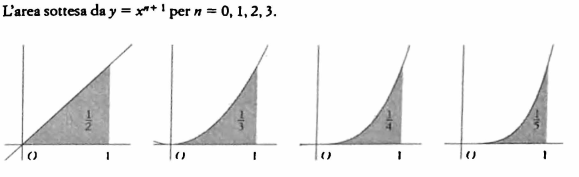
\includegraphics[scale=0.6]{Area-sotto-curve.png}
        \end{center}


    \end{block}
\end{frame}